\documentclass[11pt]{article}
\usepackage{physics}
\usepackage{graphicx}
\usepackage{tcolorbox}
\usepackage[bb=boondox]{mathalfa}
\usepackage{amsmath}
\usepackage{multicol}
\newcommand\pN{\mathcal{N}}
\usepackage{amssymb}
\usepackage{amsthm}
\usepackage{tikz}
\def\firstcircle{(90:1.75cm) circle (2.5cm)}
\def\secondcircle{(210:1.75cm) circle (2.5cm)}
\def\thirdcircle{(330:1.75cm) circle (2.5cm)}
\newcommand{\Lagr}{L}
\renewcommand{\qedsymbol}{$\blacksquare$}
\makeatletter
\newenvironment{proofw}{\par
	\pushQED{\qed}%
	\normalfont \topsep6\p@\@plus6\p@\relax
	\trivlist
	\item[]\ignorespaces
}{%
	\popQED\endtrivlist\@endpefalse
}
\makeatother

\title{\vspace{-5.0cm}University of Stockholm\\ MT7037-VT19 Statistical Information Theory\\ Final Examination }
\author{Marina Herrera Sarrias }

\begin{document}
\maketitle

\section{Exercise 1}

\begin{tcolorbox}
\textbf{(a)}
Let X and Y be discrete random variables. Show that\\
H ((X+Y)$|$X) = H(Y$|$X). Argue that if X and Y are independent then\\
H(X+Y) $\geq$ H(Y).
\end{tcolorbox}

\begin{proofw}
We wish to prove that the conditional entropy of $Z$ ($Z = g(X,Y) = X + Y$) is the same as the conditional entropy of $Y$ ($Y = Y'$ where $Y' = Z - X$) given $X$. \\

As Z is a function of $(X,Y)$ and the probability of $Z$ taking a value is linked to the probability of $X$ having one. Both probabilities are the same as $Z$ will happen if and only if X happens.

\begin{equation*}
p(Z=z|X=x) = p(Y=z-x|X=x) = p(Y=y'|X=x)
\end{equation*}

We will now prove the equality:\\
\begin{equation} \label{eq1}
\begin{split}
H(Z|X) & = \sum_{} p(x) H(Z|X=x)\\
	   & = \sum_{x \in \chi} p(X= x) \sum_{z \in \mathcal{Z}} p(Z=z|X=x) \log p(Z=z|X=x)\\
	  & = \sum_{x \in \chi} p(X= x) \sum_{y' \in \mathcal{Y'}} p(Y=y'|X=x) \log p(Y=y'|X=x)\\
	   & = \sum_{} p(x) H(Y|X=x)\\
	   & = H(Y|X)\\
\end{split}
\end{equation}

Referring to their entropy we can say that:
\begin{equation*}
 H(X,Y) = H(X) + H(Y|X) \geq  H(g(X,Y)) = H(Z) 
\end{equation*}

and consequently, knowing that conditioning reduces entropy:
\begin{equation*}
H(Z) \geq H(Z|X) = H(Y|X)  
\end{equation*}

In the case that $X$ and $Y$ are independent discrete random variables. We can say that the addition of independent random variables adds uncertainty:

\begin{equation*}
H(Z) \geq H(Z|X) = H(Y|X) = H(Y)
\end{equation*}
or similarly,
\begin{equation*}
H(Z) \geq H(Z|Y) = H(X|Y) = H(X)
\end{equation*}

So, 
\begin{equation*}
\max \{ H(X), H(Y)\} \leq H(Z)
\end{equation*}

%Furthermore, we can also say that:
%\begin{equation*}
%H(X,Y) = H(f(Z), h(Z)) \leq H(Z)
%\end{equation*}
%Finally, in case of independence, the following holds true:
%\begin{equation*}
%H(Z) = H(X) + H(Y)
%\end{equation*}
\end{proofw}
\begin{tcolorbox}
\textbf{(b)}
Show that among all\quad $N$ - valued random variables (i.e. with values
k = 1,2,...) with expected value $\mu$ ,the geometric distributed random variable
with expected value $\mu$ has the maximum value of Shannon entropy.
Reminder: The probability function in a geometric distribution is
$p(k) = {p(1 - p)}^{k-1}, k = 1,2,...$
	
\end{tcolorbox}
\begin{proofw}
Assuming that	
\begin{equation*}
P(X= k) = {p(1 - p)}^{k-1}
\end{equation*}
 Where $k$ and $X$  $\in\mathbb N_{+}$  . Knowing that:
 
\begin{minipage}{.5\linewidth}
	\begin{equation*}
	\sum_{k=1}^{+\infty} (k-1){(1-p)}^{k-1} = \frac{1-p}{{(1-(1-p))}^2}
	\end{equation*}
\end{minipage}
,
\begin{minipage}{.5\linewidth}
	\begin{equation*}
	\sum_{k=1}^{+\infty} {(1-p)}^{k-1} = \frac{1}{(1-(1-p))}\\
	\end{equation*}
\end{minipage}
 \\

The entropy of the geometric distribution is derived as: 
\begin{equation*} \label{}
\begin{split}
H(X) & = - \sum_{k=1}^{+\infty} {p(1-p)}^{k-1} \log p{(1-p)}^{k-1}\\
& = - \sum_{k=1}^{+\infty} {p(1-p)}^{k-1} \log p - \sum_{k=1}^{+\infty}(k-1){p(1-p)}^{k-1} \log (1-p)\\
& = - [\sum_{k=0}^{+\infty} {p(1-p)}^{k} \log p - \sum_{k=0}^{+\infty} k{p(1-p)}^{k} \log {(1-p)}]\\
& = -\frac{p}{1-(1-p)}\log p -\frac{(1-p)}{{(1-(1-p))}^2} \log p(1-p)\\
&= -\log p -\frac{(1-p)}{p} \log p(1-p)\\
\end{split}
\end{equation*}
We are now going to solve the maximization problem:
\begin{equation*} 
\arg \max_{p}\Big(-\sum_{k=1}^{+\infty}p_{k} \log p_{k}\Big)
\end{equation*}
Subject to the constraints: 
\begin{equation*}
\sum_{k=1}^{+\infty} p_{k} = 1
\end{equation*}

\begin{equation*}
\sum_{k=1}^{+\infty}kp_{k} = \mu
\end{equation*}
We will use the Lagrange multipliers to obtain the general form of the $p_{k}$ distribution.
\begin{equation*} 
\begin{split}
\Lagr(p_{k}, \lambda_{1}, \lambda_{2}) & = -\Big(\sum_{k=1}^{+\infty}p_{k} \log p_{k}\Big) + \lambda_{1}\Big(\sum_{k=1}^{+\infty} p_{k}-1\Big) + \lambda_{2}\Big(\sum_{k=0}^{+\infty}kp_{k}-\mu\Big)\\
\end{split}
\end{equation*}

\begin{equation*}
\begin{split}
\pdv{\Lagr}{\lambda_{1}} = 0 &= \sum_{k=1}^{+\infty} p_{k}-1\\
& = {\exp}^{(-1+\lambda_{1})} \sum_{k=1}^{+\infty} {\exp}^{(\lambda_{2})k}\\
&= {\exp}^{(-1 + \lambda_{1})}\Big(\frac{1}{1-{\exp}^{\lambda_{2}}}-1\Big) = 1\\
&= {\exp}^{(-1 + \lambda_{1})}\Big(\frac{{\exp}^{\lambda_{2}}}{1-{\exp}^{\lambda_{2}}}\Big) = 1\\
\pdv{\Lagr}{\lambda_{2}} = 0 &= \sum_{k=0}^{+\infty}kp_{k}-\mu\\
&={\exp}^{(-1+\lambda_{1})}  \sum_{k=1}^{+\infty}k {\exp}^{(\lambda_{2})k}\\
&={\exp}^{(-1+\lambda_{1})}  \frac{{\exp}^{\lambda_{2}}}{{(1-{\exp}^{\lambda_{2}})}^2} = \mu\\
\pdv{\Lagr}{p_{k}} = 0 &= - \log p_{k}-1 + \lambda_{1} +\lambda_{2}k \\
\end{split}
\end{equation*}

Where, 
\begin{equation*}
\begin{split}
\mu &= \frac{1}{1 - {\exp}^{\lambda_{2}}}\\
\lambda_{2} &= \log(\frac{\mu - 1}{\mu})\\
\lambda_{1} &= \log(\frac{1}{\mu-1})+1\\
\end{split}
\end{equation*}
Finally, the $p_{k}$ distribution is derived as:
\begin{equation}\label{lm}
\begin{split}
p_{k} &= {\exp}^{(-1 +\lambda_{1}+\lambda_{2}k)}\\
&= {\exp}^{(-1 +\lambda_{1}+\lambda_{2})}{\exp}^{(k-1)\lambda_{2}}\\
&= \frac{1}{\mu}{\exp}^{(k-1)\lambda_{2}}\\
&= \frac{1}{\mu}{\exp}^{(k-1)\log(\frac{\mu-1}{\mu})}\\
&= \Big(\frac{1}{\mu}\Big)\Big{(\frac{\mu-1}{\mu}\Big)}^{k-1}
\end{split}
\end{equation}

We also know that the mean of the geometric distribution is:
\begin{equation}\label{mean}
\begin{split}
\mu = E[X] &= \sum_{k=1}^{+\infty} k{(1-p)}^{k-1}p\\
&= p \sum_{k=1}^{+\infty} k{(1-p)}^{k-1}\\
&= p \frac{1}{{(1-(1-p))}^{2}}\\
&= \frac{1}{p}
\end{split}
\end{equation}

If we now plug the results obtained in eq.(\ref{mean}) into eq.(\ref{lm}) we can verify that $p_{k}$ is the geometric distribution i.e, the distribution that maximizes the entropy. 

We could also prove it using the Gibb's inequality eq.($\ref{GI}$),  which is just the difference of the Kullback–Leibler divergence eq.($\ref{KL}$). Knowing that the random variable $X$ distributed as $p_{k} \neq 0$ and for the random variable $Y$ distributed as $q_{k}$, where $k \in \mathbb Z^{+}$ 
\begin{equation}\label{KL}
\begin{split}
\mathbb{D}_{KL}(Y|X) &= \sum_{k=1}^{+\infty}q_{k}\log \frac{q_{k}}{p_{k}} \geq 0\\
&= \sum_{k=1}^{+\infty}q_{k}\log q_{k} - \sum_{k=1}^{+\infty}q_{k}\log p_{k}
\end{split}
\end{equation}
\begin{equation}\label{GI}
- \sum_{k=1}^{+\infty}q_{k}\log q_{k} \leq - \sum_{k=1}^{+\infty}q_{k}\log p_{k}
\end{equation}
and knowing that:
\begin{equation*}
H(Y) = - \sum_{k=1}^{+\infty}q_{k}\log q_{k}
\end{equation*}
\begin{equation*}
\begin{split}
- \sum_{k=1}^{+\infty}q_{k}\log p_{k} &= - \sum_{k=1}^{+\infty}q_{k}(\log p + (1-k) \log (1-p))\\
&= - \log p\sum_{k=1}^{+\infty}q_{k} -\sum_{k=1}^{+\infty} q_{k}(1-k) \log (1-p))\\
&= - \log p -\sum_{k=1}^{+\infty} q_{k}(1-k) \log (1-p)\\
&= - \log p -\log (1-p) \sum_{k=1}^{+\infty} q_{k}(1-k)\\
&= - \log p -\log (1-p) \sum_{k=1}^{+\infty} q_{k} + \log (1-p) \sum_{k=1}^{+\infty} k q_{k}\\
&= - \log p -\log (1-p) + \log (1-p) \sum_{k=1}^{+\infty} k q_{k}\\
&= - \log p -\log (1-p) + \log (1-p) \mathbb{E}[Y] \\
&= - \log p +\log (1-p) (\mathbb{E}[Y]-1) \\
&= -\log p -\frac{(1-p)}{p} \log p(1-p) = \mathbb{H}(X)\\
\end{split}
\end{equation*}

\begin{equation*}
\mathbb{H}(Y) \leq \mathbb{H}(X)  
\end{equation*}


\end{proofw}

\begin{tcolorbox}
\textbf{(c)}
Show that\\
$(i)$ H($X_{1}$,$X_{2}$,$X_{3}$) $\leq$ $\frac{1}{2}$ [H($X_{1}$,$X_{2}$) +H($X_{2}$,$X_{3}$) +H($X_{1}$,$X_{3}$)]\\

$(ii)$H($X_{1}$,$X_{2}$,$X_{3}$) $\geq$ $\frac{1}{2}$ [H($X_{1}$,$X_{2}$ $|$$X_{2}$)+H($X_{2}$,$X_{3}$$|$$X_{1}$)+H($X_{1}$,$X_{3}$$|$$X_{2}$)]\\

\end{tcolorbox}
Using the chain rule of entropy we can prove that a collection of random variables are the sum of the conditional entropies, such that:

\begin{equation*}
H(X_{1},X_{2},...,X_{n}) = \sum_{i=1}^{n} H(X_{i}|X_{i-1},...,X_{1})\\
\end{equation*}

We also know that as conditioning reduces entropy:
\begin{equation*}
H(X_{n})\geq H(X_{n}|X_{1}) \geq H(X_{n}|X_{n-1},X_{1})
\end{equation*}
\begin{proofw}
(i)\\

The left hand side of the inequality is:

\begin{equation}\label{LHS}
\begin{split}
H(X_{1},X_{2},X_{3}) & = H(X_{1}) + H(X_{2},X_{3}|X_{1}) \\
& = H(X_{1}) + H(X_{2}|X_{1}) + H(X_{3}|X_{2},X_{1})\\
\end{split}
\end{equation}

While , the right hand side is:
\begin{equation}\label{RHS}
\begin{split}
H(X_{1},X_{2})+H(X_{2},X_{3})+H(X_{1},X_{3}) & = H(X_{1}) + H(X_{2}|X_{1}) + H(X_{2})\\
&= + H(X_{3}|X_{2}) + H(X_{1}) + H(X_{3}|X_{1})\\
&= 2H(X_{1}) + H(X_{2}|X_{1}) + H(X_{2})\\
&= + H(X_{3}|X_{2}) + H(X_{3}|X_{1})
\end{split}
\end{equation}

Now, referring to the results obtained in eq.($\ref{RHS}$) we could also say that:

\begin{equation}\label{proveRHS}
\begin{split}
\frac{1}{2}[H(X_{2})+ H(X_{2}|X_{1})+\\H(X_{3}|X_{2})+H(X_{3}|X_{1})] &\geq  + \frac{1}{2}[H(X_{2}|X_{1})+H(X_{2}|X_{1})+\\ & H(X_{3}|X_{2},X_{1} )+H(X_{3}|X_{2}, X_{1})]\\
&\geq H(X_{2}|X_{1}) + H(X_{3}|X_{2},X_{1} )
\end{split}
\end{equation}

and, because of the above, we can finally prove that:
\begin{equation*}
H(X_{1},X_{2},X_{3}) \leq H(X1) + \frac{1}{2}[H(X_{2})+ H(X_{2}|X_{1})+\\H(X_{3}|X_{2})+H(X_{3}|X_{1})]
\end{equation*}

\end{proofw}

\begin{proofw}
	$(ii)$\\
	
The left hand side of the inequality is the same as in eq.($\ref{LHS}$) while the right hand side is as follows:
\begin{equation}\label{LHSii}
\begin{split}
 &= \frac{1}{2} [H(X_{1},X_{2}|X_{3})+H(X_{2},X_{3}|X_{1})+H(X_{1},X_{3}|X_{2})]\\
& = \frac{1}{2}[H(X_{1}|X_{3})+H(X_{2}|X_{3},X_{1})+H(X_{2}|X_{1})
\\&+H(X_{3}|X_{2},X_{1})+H(X_{1}|X_{2})+H(X_{3}|X_{2},X_{1})]\\
& = H(X_{3}|X_{2},X_{1}) + \frac{1}{2} [H(X_{1}|X_{3})+H(X_{2}|X_{3},X_{1})\\
&+H(X_{2}|X_{1})+H(X_{1}|X_{2})]\\
\end{split}
\end{equation}	

Following the same intuition as in eq.($\ref{proveRHS}$) we can say about the results obtained in eq.($\ref{LHSii}$) that:

\begin{equation*}
\begin{split}
\frac{1}{2} [H(X_{1}|X_{3})+H(X_{2}|X_{3},X_{1})\\+H(X_{2}|X_{1})+H(X_{1}|X_{2})] &\leq \frac{1}{2}[H(X_{2}|X_{1})+H(X_{2}|X_{1}) + H(X_{1}) + H(X_{1})]\\
& \leq H(X_{1}) + H(X_{2}|X_{1})\\
\end{split}
\end{equation*}	

We can now verify that:

\begin{equation*}
\begin{split}
H(X_{1},X_{2},X_{3}) &\geq H(X_{3}|X_{2},X_{1}) + \frac{1}{2} [H(X_{1}|X_{3})+H(X_{2}|X_{3},X_{1}) \\&+H(X_{2}|X_{1})+H(X_{1}|X_{2})]\\
\end{split}
\end{equation*}	
\end{proofw}
\pagebreak
\begin{tcolorbox}
\textbf{(d)}
Suppose that $(X ,Y ,Z)$ are jointly normal distributed and that
$X \rightarrow Y \rightarrow Z \rightarrow$ forms a Markov chain. Let X and Y have the correlation coefficient $\rho1$ and let Y and Z have the correlation coefficient $\rho2$. Find mutual information $I(X;Z)$.
\end{tcolorbox}
\begin{proofw}
The mutual information $I(X;Z)$ is the reduction in the uncertainty of $X$ due to the knowledge of $Z$ and it is represented as:
\begin{equation}\label{eq2}
\begin{split}
I(X;Z) & = H(X) + H(Z) - H(X, Z)\\
       & = H(X) + H(X|Z)\\
\end{split}
\end{equation}

Furthermore the entropy of a normal distribution is derived as:
\begin{equation*}
h(X)  = -\int_{-\infty}^{\infty} \phi(X) \log \phi(X) dx\\
\end{equation*}

Where the density function $\phi(X)$ is:

\begin{equation}\label{eq3}
\phi(X) = \frac{1}{\sqrt{2\pi {\sigma}^2}} \cdot {\exp}^\frac{{-(x-\mu)}^2}{2 {\sigma}^2}\\
\end{equation}

and then, plugging eq.(\ref{eq3}) in eq.(\ref{eq2}) we obtain:

\begin{equation*}
\begin{split}
h(X)  &= -\int_{-\infty}^{\infty} \phi(X) \log (\frac{1}{\sqrt{2\pi {\sigma}^2}} \cdot {e}^\frac{{-(x-\mu)}^2}{2 {\sigma}^2}) dx\\
	  &= -\int_{-\infty}^{\infty} \phi(X) \log \frac{1}{\sqrt{2\pi {\sigma}^2}} dx + \log (e) \int_{-\infty}^{\infty} \phi(X)(\frac{{-(x-\mu)}^2}{2 {\sigma}^2})  dx  \\
	  &= -\int_{-\infty}^{\infty} \phi(X) \log \frac{1}{\sqrt{2\pi {\sigma}^2}} dx - \log (e) \frac{1}{2{\sigma}^2} \int_{-\infty}^{\infty} {(x-\mu)}^2 \phi(X)dx  \\
	  &= \frac{1}{2} \log (2\pi{\sigma}^2) - \log e \frac{1}{2}\\
	  &= \frac{1}{2} [\log 2\pi{\sigma}^2 - \log e]\\
	  &= -\frac{1}{2}\log[ 2\pi e {\sigma}^2]\\	  
\end{split}
\end{equation*}

Since $(X,Y,Z)$ are jointly normal distributed $X$ and $Z$ will also be. Their covariance matrix $\Sigma_{x,z}$ is defined as:
\[
\Sigma_{x,z} =
\begin{bmatrix}
{\sigma_{x}}^2 & \sigma_{x}\sigma_{z}\rho_{xz} \\
\sigma_{x}\sigma_{z}\rho_{xz} & {\sigma_{z}}^2\\
\end{bmatrix}
\]

Now, going back to the mutual information $I(X;Z)$ defined on eq.(\ref{eq2}) we obtain:

\begin{equation*}
\begin{split}
I(X;Z) & = \frac{1}{2}\log(2\pi e {\sigma_{x}}^2) + \frac{1}{2}\log(2\pi e {\sigma_{z}}^2) - \frac{1}{2}\log({2\pi e }^2|\Sigma_{x,z}|)\\
	&= \frac{1}{2}\log(2\pi e {\sigma_{x}}^2) + \frac{1}{2}\log(2\pi e {\sigma_{z}}^2) - \log(2\pi e ) - \frac{1}{2}|\Sigma_{x,z}|\\
\end{split}
\end{equation*}
therefore;
\begin{equation*}
\begin{split}
I(X;Z) & =  - \frac{1}{2}|\Sigma_{x,z}|
\end{split}
\end{equation*}
Where,
\begin{equation*}
\begin{split}
|\Sigma_{x,z}| & = {\sigma_{x}}^2 {\sigma_{z}}^2 - {\sigma_{x}}^2{\sigma_{z}}^2{\rho_{xz}}^2\\
			& = {\sigma_{x}}^2{\sigma_{z}}^2(1-{\rho_{xz}}^2)\\
\end{split}
\end{equation*}

If we now assume that $(X,Y,Z)$ $\sim$ $\pN(0,1)$:

\begin{equation}\label{eq5}
\begin{split}
I(X;Z) & =  -\frac{1}{2}\log	(1 - {\rho_{xz}}^2)\\
\end{split}
\end{equation}

The Markov chain $X \rightarrow Y \rightarrow Z $ implies that the conditional distribution of $Z$ depends only on $Y$ and is conditionally independent of $X$. The joint probability of the random variables $(X, Y, Z)$ is:
\begin{equation*}
p(x,y,z) = p(x)p(y|x)p(z|y)
\end{equation*}
and it implies conditional independence as:
\begin{equation}\label{eq4}
\begin{split}
p(x,z|y) & = \frac{p(x,y,z)}{p(y)}\\
		& = \frac{p(x)p(x|y)p(z|y)}{p(y)}\\
		& = \frac{p(x,y)p(z|y)}{p(y)}\\
		& = \frac{p(x|y)p(y)p(z|y)}{p(y)}\\
		& = p(x|y)p(z|y)
\end{split}
\end{equation}
 
\pagebreak
Then the correlation coefficient $\rho_{xz}$ is obtained as:
\begin{equation*}
\begin{split}
\rho_{xz} & = \frac{E[XZ]-E[X]E[Z]}{\sigma_{x}\sigma_{z}}\\
		  & =\frac{E[XZ]}{\sigma_{x}\sigma_{z}}\\
		  & =\frac{E[E[XZ|Y]]}{\sigma_{x}\sigma_{z}}\\
		  & =\frac{E [E[X|Y] E[Z|Y]]}{\sigma_{x}\sigma_{z} }\\
		  & =\frac{E[\frac{E[Y]-E[X]cov(X,Y)}{\sigma_{y}} + \frac{cov(X,Y)}{\sigma_{y}}Y][\frac{E[Y]-E[Z]cov(Z,Y)}{\sigma_{y}}+ \frac{cov (Z,Y)}{\sigma_{y}}Y] } {\sigma_{x}\sigma_{z}}\\
		  & =\frac{E[ \frac{cov(X,Y)}{\sigma_{y}}Y][\frac{cov (Z,Y)}{\sigma_{y}}Y]} {\sigma_{x}\sigma_{z}}\\
		  &=\frac{E[\sigma_{x}\rho_{xy}Y][\sigma_{z}\rho_{zy}Y]}{\sigma_{x}\sigma_{z}}\\
		  &=\rho_{xy}\rho_{zy}E[{Y}^{2}]\\
		  &=\rho_{xy}\rho_{zy}
\end{split}
\end{equation*}
Plugging the results into eq.(\ref{eq5}), we can now conclude that:

\begin{equation*}
\begin{split}
I(X;Z) & =  -\frac{1}{2}\log	(1 - {\rho_{xy}}^2{\rho_{zy}}^2)\\
	& =  -\frac{1}{2}\log	(1 - {\rho_{1}}^2{\rho_{2}}^2)\\
\end{split}
\end{equation*}
\end{proofw}
\pagebreak

\section{Exercise 2}
\begin{tcolorbox}
\textbf{(a)}
Define the transfer entropy, starting from Schreiber’s definition in
Phys. Rev. Lett., 85, 461, 2000, in terms of mutual information and Shannon
entropy.
\end{tcolorbox}

The random time series processes $\mathbb {X}^{(k)}_{t}$ and $\mathbb {Y}^{(l)}_{t}$ are a join of sequential processes that evolve over time $t$, with a history length (lags/time steps) of $k$ for the target variable and $j$ for the source variable, in which most of the cases $l=1$ or $l=k$.
\begin{equation*}
\begin{split}
\mathbb {X}^{(k)}_{t} &= (X_{t}, X_{t-1},...,X_{t-k+1})\\
\mathbb {Y}^{(l)}_{t} &= (Y_{t}, Y_{t-1},...,Y_{t-l+1})
\end{split}
\end{equation*}
The transfer entropy ${T}^{(k,l)}_{\mathbb{Y}\rightarrow \mathbb{X}}(t)$ is defined as the difference between the entropy of the state of $X_{t}$ conditioned on its own past ${\mathbb{X}}^{k}_{t-1}$ and its entropy conditioned in addition to the past of ${\mathbb{Y}}^{l}_{t-1}$. It therefore measures how much information the source variable ${\mathbb{Y}}^{l}_{t-1}$ provides about the state transitions in the target variable ${\mathbb{X}}^{k}_{t-1}$. It measures the deviation in bits from the Markov property of conditional independence. 

\begin{equation*}
{T}^{(k,l)}_{\mathbb{Y}\rightarrow \mathbb{X}}(t) = H(X_{t}|{\mathbb{X}}^{k}_{t-1}) - H(X_{t}|{\mathbb{X}}^{k}_{t-1},{\mathbb{Y}}^{l}_{t-1})
\end{equation*}


It can also be formulated as the conditional mutual information: \\
$I(X_{t}, {\mathbb{Y}_{t-1}}^{(l)}|{\mathbb{X}_{t-1}}^{(k)})$ which is the reduction of uncertainty by the process ${\mathbb{Y}_{t-1}}^{(l)}$ in the state $X_{t}$ conditioned to its own past. i.e, how much information the source variable ${\mathbb{X}_{t-1}}^{(k)}$ adds in predicting the next state of the target variable. The current state of $X_{t}$ will depend probabilistically on the state of $Y_{t-1}$ at the previous time step $t-1$.  \\

\begin{tcolorbox}
\textbf{(b)}
Why is mutual information not a good measure for an information transfer?
\end{tcolorbox}

Mutual information neither contains dynamical nor directional information. Directional in the sense that for: $I(X_{t}:Y_{t})$ the exchange between the two systems is a symmetric measure of statically shared information. i.e, we do not know if there is a direction. We will only know that if the mutual information is greater than zero the two variables are not independent. While in a directional system there is only information transfer in one direction $Y \rightarrow X$ as the information transfer in $X \rightarrow Y$ will be zero. \\ 

Dynamical, in the sense that mutual information is a property of static probability distributions and a dynamic system is described as the evolution of a set of state variables, i.e a system that evolves over time. Conditioning on the past can make a measure to be directional, and dynamic, which is the case of the transfer entropy. The Cellular Automata is a good example of a directional and dynamic system.\\

%even though the introduction of a time lag in one of the variables such that $I(X_{t}:Y_{t-s})$ can add directional information to the mutual information, although it still fails to take into account shared history between the processes.\\

%Transfer entropy takes the mutual information properties and in addition takes the dynamics of information transport into account, where we will be able to quantify the exchange of information between two systems separetly and on both directions, it could also be conditioned to common input signals. \\
	
\begin{tcolorbox}
\textbf{(c)}
Does Schreiber’s definition of transfer entropy coincide with the
definition of mutual information?
\end{tcolorbox}
\begin{proofw}


Yes, it coincides with the definition of conditional mutual information, it can be proved as following:

\begin{equation}\label{transfentropy}
\begin{split}
{T}^{(k,l)}_{\mathbb{Y}\rightarrow \mathbb{X}}(t) &= \sum_{X_{t}, {\mathbb{X}_{t-1}}^{(k)},{\mathbb{Y}_{t-1}}^{(l)}} p(x_{t}, {\mathbb{x}_{t-1}}^{(k)},{\mathbb{y}_{t-1}}^{(l)}) \log \frac{p(x_{t}|{\mathbb{x}_{t-1}}^{(k)},{\mathbb{y}_{t-1}}^{(l)})}{p(x_{t}|{\mathbb{x}_{t-1}}^{(k)})}
\end{split}
\end{equation}
Where: 
\begin{equation}\label{proofcp}
\begin{split}
p(x_{t}|{\mathbb{x}_{t-1}}^{(k)},{\mathbb{y}_{t-1}}^{(l)}) &= \frac{p(x_{t},{\mathbb{x}_{t-1}}^{(k)},{\mathbb{y}_{t-1}}^{(l)}) }{p({\mathbb{x}_{t-1}}^{(k)},{\mathbb{y}_{t-1}}^{(l)})}\\
&= \frac{p(x_{t},{\mathbb{y}_{t-1}}^{(l)}|{\mathbb{x}_{t-1}}^{(k)}) p({\mathbb{x}_{t-1}}^{(k)})} {p({\mathbb{x}_{t-1}}^{(k)},{\mathbb{y}_{t-1}}^{(l)})}\\
&=\frac{p(x_{t},{\mathbb{y}_{t-1}}^{(l)}|{\mathbb{x}_{t-1}}^{(k)})}{\frac{p({\mathbb{x}_{t-1}}^{(k)},{\mathbb{y}_{t-1}}^{(l)})}{p({\mathbb{x}_{t-1}}^{(k)})}}\\
&= \frac{p(x_{t},{\mathbb{y}_{t-1}}^{(l)}|{\mathbb{x}_{t-1}}^{(k)})} {p({\mathbb{y}_{t-1}}^{(l)}|{\mathbb{x}_{t-1}}^{(k)})}\\
\end{split}
\end{equation}

Plugging the results of eq.($\ref{proofcp}$) into eq.($\ref{transfentropy}$) we obtain:
\begin{equation*}
\begin{split}
{T}^{(k,l)}_{\mathbb{Y}\rightarrow \mathbb{X}}(t) &= \sum_{X_{t}, {\mathbb{X}_{t-1}}^{(k)},{\mathbb{Y}_{t-1}}^{(l)}} p(x_{t}, {\mathbb{x}_{t-1}}^{(k)},{\mathbb{y}_{t-1}}^{(l)}) \log \frac{p(x_{t},{\mathbb{y}_{t-1}}^{(l)}|{\mathbb{x}_{t-1}}^{(k)})}{p(x_{t}|{\mathbb{x}_{t-1}}^{(k)})p({\mathbb{y}_{t-1}}^{(l)}|{\mathbb{x}_{t-1}}^{(k)})}
\end{split}
\end{equation*}
And knowing that the mutual information $I(X_{t}, {\mathbb{Y}_{t-1}}^{(L)}|{\mathbb{X}_{t-1}}^{(k)})$ is:

\begin{equation*}\label{mutual_information}
\begin{split}
I(X_{t}, {\mathbb{Y}_{t-1}}^{(L)}|{\mathbb{X}_{t-1}}^{(k)}) &= \sum_{X_{t}, {\mathbb{X}_{t-1}}^{(k)},{\mathbb{Y}_{t-1}}^{(l)}} p({X_{t}, {\mathbb{X}_{t-1}}^{(k)},{\mathbb{Y}_{t-1}}^{(l)}}) \log\frac{p(x_{t}, {\mathbb{y}_{t-1}}^{(l)}|{\mathbb{x}_{t-1}}^{(k)})}{p(x_{t}|{\mathbb{x}_{t-1}}^{(k)}) p({\mathbb{y}_{t-1}}^{(l)}|{\mathbb{x}_{t-1}}^{(k)})}\\
\end{split}
\end{equation*}

We can now verify that:
\begin{equation*}
\begin{split}
{T}^{(k,l)}_{\mathbb{Y}\rightarrow \mathbb{X}}(t)  = I(X_{t}, {\mathbb{Y}_{t-1}}^{(l)}|{\mathbb{X}_{t-1}}^{(k)}) 
\end{split}
\end{equation*}
\end{proofw}
\begin{tcolorbox}
\textbf{(d)}
What is the meaning of local transfer entropy?
\end{tcolorbox}

The local transfer entropy describes the information contained in the source variable $y_{t-1}$ about the next state $x_{t}$ at a time $t$ and that is not contained in ${x}^{(k)}_{t-1}$ , as this is a local measure it is defined at each time $t$. The average over all the points will be the transfer entropy of the system. \\

The local transfer entropy gives information about the dynamics (transition probabilities) of information transfer in time. Insights that the transfer entropy can not access, as it is an average. It can also be defined as a local conditional mutual information: $i( {\mathbb{y}_{t-1}}^{(l)};x_{t}|{\mathbb{x}_{t-1}}^{(k)})$.\\

\begin{tcolorbox}
\textbf{(e)}
Is the Granger causality concept the same as transfer entropy?
Explain possible similarities and differences.
\end{tcolorbox}
According to the paper by Barnett et al., the concepts od Granger causality and transfer entropy are entirely equivalent for Gaussian processes, up to certain conditions and under a parametric formulation. It is important to stress in the fact that they will only measure the same thing for Gaussian processes. \\

Both concepts numerical equivalence will depend on the method used to estimate the transfer entropy in the sample. i.e, if conditional entropies are estimated directly from sample probability distributions, results will vary,therefore the Granger causality can be considered after the introduction of constraints in the data, i.e Granger parametric formulation.  \\

Some of this equivalence formulations are:
Granger causality and transfer entropy for discrete variables with jointly multivariate Gaussian distribution are equivalent up to a factor of two,this as the Granger transfer entropy general formulation only deals with univariate variables, so this is just the result of the formulation extension by adding an extra conditioning factor. On the other hand, for discrete random variables with jointly multivariate Weinman exponential distribution, the Granger causality and transfer entropy will be the same up to a factor of 1. And for discrete random variables with jointly multivariate log-normal distribution, the Granger causality and transfer entropy will also be the same, up to a factor of $\frac{1}{2}$\\

The possible advantages that either measure could have are strongly related with the data and its underlying stochastic generative process. For instance, For highly non-linear data where there is too much variability, this can lead to invalidate the residuals-regressors un-correlation assumption (eq.(5) in the paper), same for a given case in which the regressors used for modeling do not have sufficient explanatory power, all of these could lead to compromise the statistical inference. So, indifferently that our data satisfies, the conditions for formulation a linear model this does not mean that the results will be significant, and that the parsimonious principal will hold, and therefore there will be occasions in which it will be better a non parametric  method (TE). \\


\begin{tcolorbox}
\textbf{(f)}
To complete this part you need to read the paper by Lizier and Prokopenko in Eur. Phys. J. B 73, 605-615, 2010.\\
$i)$  Does information transfer have the same meaning as information flow in the opinion of the authors of the paper? Explain possible similarities and differences.\\
$ii)$ What is the difference between interventional and standard
conditional probabilities?\\
$iii)$ Explain the difference between local transfer entropy and local information flow.\\
$iv)$What are the advantages of the definition of local information flow according to the authors of the paper.\\
\end{tcolorbox}
$(i)$\\

The thesis of the paper is that both concepts, are different, and should be considered separately.\\

The information flow is principally related to identifying up to what extent the source variable can influence on predicting the next state of the target variable, while the predictive information transfer refers to how the state of the source variable helps on predicting the next state of the target variable. i.e, in which amount the source variable contributes to the prediction. \\

Both measures are also done differently, information transfer is quantified by transfer entropy, which only takes into account local values (observed conditional correlations), while information flow is quantified by introducing certain intervention or deviation, so we can actually learn in which extent the source variable influences the state of the target variable.\\

The argument for defining local information transfer and local information flow is the same however the meaning in local information flow is different. Also, unlike information transfer, information flow is not an average of local values.\\

%Both measures can actually be complementary, including the conditions under which they converge.

%The predictive information transfer can be used to describe the emergent computation on the target variable i.e, this information is being transferred to the computation taking place at the target variable. \\

%Information transfer refers to the amount of information the source variable contributes to the next state of the target variable, i.e knowing the state of the source variable how much will this help in predicting the next state of the target variable.\\

%On the other hand, information flow refers to the direct influence that the source variable might have on predicting the next state of the target variable. i.e, if we change the status of the source variable, how much would this affect in predicting the next status of the target variable. Therefore in order to determine this influence, it is necessary to introduce certain intervention or deviation, so we can actually learn in which extent the source variable influences the state of the target variable. \\

$(ii)$\\

Following the paper's definition, considering two variables $s$ and $a$ an interventional conditional probability $p(a|\tilde{s})$ considers the distribution of $a$ resulting from imposing the value of $\tilde{s}$, while its correlation alters $p(a|s)$ generally by $p(a)$, meaning that imposing a value on $s$, has no effect. I will illustrate this with a simple example. Lets say we have a disease  $s$ ("a weird disease"), which is correlated with $a$ ("shortness of breath"), in the sense that $s$ can cause $a$.  If we ask about the probability of suffering from shortness of breath given that we intervened having this weird disease. The intervention wont have any effect on the relevant causal link, so it will be the same as the conditional probability: 
\begin{equation*}
p(a|\tilde{s})  = P(a|s)
\end{equation*}
Now, we also know that, $s$ and $a$ are solely caused by $g$ ("certain bacterial infection"). If the system of $s$ is intervened to set the value of this variable, so the question will be now: what is the probability of suffering from shortness of breath if I eliminate having the weird disease using a magic potion? such that:
\begin{equation*}
P(a|\tilde{s})  = P(a)
\end{equation*}
This will be the same as the prior probability of suffering from shortness of breath. This, as having the weird disease has been disconnected from suffering from shortness of breath, thus it does not provide any information about it.\\

%information flow is measured via  interventional and standard conditional probabilities.
 $(iii)$\\
 
The local information flow is defined in a similar manner as the local transfer entropy. However the local information flow has a different meaning. Let's say that given the observation $(y, x, \boldsymbol{s})$, we study the local cause effect of $y$ on $x$ given the imposition $\tilde{s}$ of the same observation. The local information flow will finally be the average over the product of interventional conditional probabilities $p(s) p(y|\boldsymbol{\tilde{s}}) p(x|\tilde{y},\boldsymbol{\tilde{s}})$.\\

As there is a possibility that not all of the tuples $\{y,x,s\}$ will actually be observed, we still need to take into account all the unobserved tuples as they still have a valuable weight. Therefore we should not rely only in the observed values, we should take into account all possible combinations so we can understand the causation in our system.\\

In summary, the local information flow does not make reference to a certain observation given a moment in time  $t$, if not, it is related to how the general configuration of $(y, x, \boldsymbol{s})$ is attributed to the given observation at the given time step.\\

$(iv)$\\

Although both measures are complementary, the main advantage could rely on the fact that the measure for transfer entropy does not detect all causal effects that information flow does. so, in order to measure information transfer, the transfer entropy should only be applied to causal information sources, for a given target variable. Otherwise it will just be a measure of correlations.

\pagebreak
\section{Exercise 3}

To understand better the concepts of multi-information and its decomposition, this exercise requires you to work out some details in the paper by Schneidman et al., Phys. Rev. Lett., 91, 238701, 2003 discussed in the class.\\
	

\begin{tcolorbox}
\textbf{(b)}
Can you derive $Eq. (8)$ of the paper and correct the typos? Hint: Use the
Venn diagram. This exercise shows that 1) although the area-information
correspondence of the Venn diagram does not hold in the 3-variable case, the Venn
diagram is still useful when deriving relations between different information
quantities; 2) mistakes exist in published papers, so always be critical in reading them.\\
\end{tcolorbox}

\begin{figure}[h!]
	\centering
	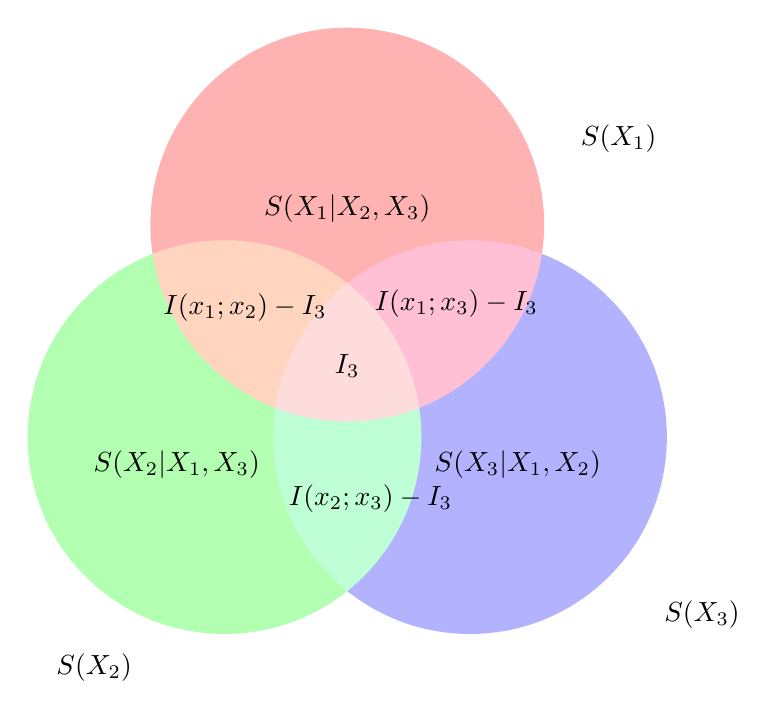
\begin{tikzpicture}
	\begin{scope}[blend group=soft light]
	\fill[red!30!white]   ( 90:1.8) circle (2.5);
	\fill[green!30!white] (210:1.8) circle (2.5);
	\fill[blue!30!white]  (330:1.8) circle (2.5);
	\end{scope}
	\node at ( 90:2)    {$S(X_{1}|X_{2},X_{3})$};
	\node at ( -35:5.5)    {$S(X_{3})$};
	\node at ( 40:4.5)    {$S(X_{1})$};
	\node at ( 50:-5)    {$S(X_{2})$};
	\node at (210:2.5)    {$S(X_{2}|X_{1},X_{3})$};
	\node at (330:2.5)    {$S(X_{3}|X_{1},X_{2})$};
	\node(0,0) {$I_{3}$};
	\draw(30:1.6cm) node {$I(x_{1};x_{3})-I_{3}$};
	\draw(150:1.5cm) node {$I(x_{1};x_{2})-I_{3}$};
	\draw(280:1.7cm) node {$I(x_{2};x_{3})-I_{3}$};
	\end{tikzpicture}
	\caption{Venn diagram of triplet information}
	\label{fig:ven}
\end{figure}
\pagebreak
\begin{proofw}
	
	From the Venn diagram in Figure($\ref{fig:ven}$) we can derive the value of $I_{3}$ as follow:
\begin{equation}\label{entr}
\begin{split}
I_{3} &= S(X_{1},X_{2},X_{3}) - S(X_{1}|X_{2},X_{3}) - S(X_{2}|X_{1},X_{3})- S(X_{3}|X_{2},X_{1})\\
& - [I(X_{1};X_{3})- I_{3}] -  [I(X_{2};X_{3})-I_{3}] - [I(X_{1};X_{2})-I_{3}]\\
&= S(X_{1},X_{2},X_{3}) - S(X_{1}|X_{2},X_{3}) - S(X_{2}|X_{1},X_{3})- S(X_{3}|X_{2},X_{1})\\
& - I(X_{1},X_{2}|X_{3}) - I(X_{1},X_{3}|X_{2})  - I(X_{2},X_{3}|X_{1})\\
&= S(X_{1},X_{2},X_{3}) - [S(X_{1},X_{2},X_{3})-S(X_{2},X_{3})] - [S(X_{1},X_{2},X_{3})-S(X_{1},X_{3})] \\
& - [S(X_{1},X_{2},X_{3})-S(X_{2},X_{1})] - I(X_{1},X_{2}|X_{3}) - I(X_{1},X_{3}|X_{2})  - I(X_{2},X_{3}|X_{1})\\
&= S(X_{1},X_{2},X_{3}) - 3 S(X_{1},X_{2},X_{3}) +S(X_{2},X_{3}) + S(X_{1},X_{3}) + S(X_{2},X_{1}) \\
& + 3 S(X_{1},X_{2},X_{3}) -2S(X_{2},X_{3}) -2S(X_{2},X_{1}) -2S(X_{1},X_{3}) +S(x_{1})+S(x_{2})+S(x_{3})\\
&= S(X_{1},X_{2},X_{3}) -S(X_{2},X_{3}) - S(X_{1},X_{3}) - S(X_{1},X_{2}) + S(X_{1})+S(X_{2})+S(X_{3})\\
&= \sum_{i}S(X_{i}) - \sum_{i<j}S(X_{i},X_{j}) + S(X_{1},X_{2},X_{3})
\end{split}
\end{equation}

The results obtained in eq.(\ref{entr}) agree with the one derived in the first line of $eq(8)$ in the paper. I will now proceed to prove it referring to the mutual information where:
\begin{equation*}
\begin{split}
\sum_{i<j}I(X_{i},X_{j}) - I(X_{1},X_{2},X_{3}) &= [I(X_{1},X_{3})+I(X_{2},X_{3})] - I(\{X_{1},X_{2}\};X_{3})
\end{split}
\end{equation*}

We also know that:
\begin{equation*}
\begin{split}
 I(\{X_{1},X_{2}\};X_{3})& = \sum_{X_{1},X_{2},X_{3}}p(X_{1},X_{2},X_{3})\log\frac{p(X_{1},X_{2},X_{3})}{p(X_{1},X_{2})p(X_{3})}\\
 & = H(X_{3}) - H(X_{3}|X_{1},X_{2}) \\
 & = H(X_{3}) + H(X_{1},X_{2}) - H(X_{1},X_{2},X_{3})  
\end{split}
\end{equation*}

\begin{equation*}
\begin{split}
\sum_{i<j}I(X_{i},X_{j}) - I(X_{1},X_{2},X_{3}) & = [I(X_{1},X_{3})+I(X_{2},X_{3})] - [H(X_{3}) + H(X_{1},X_{2}) - H(X_{1},X_{2},X_{3}) ]\\
&=[H(X_{1})+ H(X_{3}) - H(X_{1},X_{3})]+[H(X_{2}) + H(X_{3})\\ &-H(X_{2},X_{3})] - H(X_{3}) - H(X_{1},X_{2}) + H(X_{1},X_{2},X_{3}) \\
&=[H(X_{1})+ H(X_{2}) + H(X_{3}) - H(X_{1},X_{3})- H(X_{2},X_{3})\\
& - H(X_{1},X_{2}) + H(X_{1},X_{2},X_{3})\\
&=\sum_{i}S(X_{i}) - \sum_{i<j}S(X_{i},X_{j}) + S(X_{1},X_{2},X_{3})
\end{split}
\end{equation*}

We can now verify that:

\begin{equation*}
\sum_{i}S(X_{i}) - \sum_{i<j}S(X_{i},X_{j}) + S(X_{1},X_{2},X_{3}) = \sum_{i<j}I(X_{i},X_{j}) - I(X_{1},X_{2},X_{3})
\end{equation*}

And point out that there is an error of signs in the paper, where the right formulation is : $\sum_{i<j}I(X_{i},X_{j}) - I(X_{1},X_{2},X_{3})$ instead of $I(X_{1},X_{2},X_{3}) - \sum_{i<j}I(X_{i},X_{j})$.\\

On the other hand, representing three terms entropies using the $Venn$ diagram can be misleading. Mostly as entropies can be confused with probabilties, and by the misconception that all regions correspond to positive quantities, which could be not case. (it is for a two entropy representation)
\end{proofw}

\begin{tcolorbox}
\textbf{(c)}
Show that the connected information of order k in $Eq. (6)$ of the paper
can be written as a relative entropy. When does it equal to zero?
\end{tcolorbox}

The connected information of order $k$ (subset of $k$ elements of $N$ variables) is the information gain when we go from knowing only the marginals of order $k-1$ to knowing also the marginals of order $k$. It is defined as:
\begin{proofw}
\begin{equation*}
{I}^{(k)}_{C}(\{x_{i}\}) = S[{\tilde{P}}^{(k-1)}(\{x_{i}\})] - S[{\tilde{P}}^{(k)}(\{x_{i}\})]
\end{equation*}
Considering $N$ variables $\{x_{i}\}$, where $i = 1,2,3$
\begin{equation*}
\begin{split}
{I}^{(2)}_{C}(\{x_{i}\}) &= S[{\tilde{P}}^{(1)}(\{x_{i}\})] - S[{\tilde{P}}^{(2)}(\{x_{i}\})]\\
 &= S[{\tilde{p}}^{(1)}(x_{1}, x_{2}, x_{3})] - S[{\tilde{p}}^{(2)}(x_{1}, x_{2}, x_{3})]\\
  &= S[p(x_{1})p(x_{2})p(x_{3})] - S[p(x_{1},x_{2},x_{3})]\\ 
  &= \sum p(x_{1},x_{2},x_{3}) \log p(x_{1},x_{2},x_{3}) - \sum p(x_{1},x_{2},x_{3}) \log p(x_{1})p(x_{2})p(x_{3})  \\ 
  &= \sum p(x_{1},x_{2},x_{3}) \frac{\log p(x_{1},x_{2},x_{3}) }{p(x_{1})p(x_{2})p(x_{3})}\\ 
   &= D_{KL}(p(x_{1},x_{2},x_{3})||(p(x_{1})p(x_{2})p(x_{3}))) \\ 
  &= D_{KL}{\tilde{P}}^{(2)}(\{x_{i}\})||{\tilde{P}}^{(1)}(\{x_{i}\})) \\ 
  &= D_{KL}({\tilde{P}}^{(k)}(\{x_{i}\})||{\tilde{P}}^{(k-1)}(\{x_{i}\})) \geq 0 \\ 
\end{split}
\end{equation*}
If the result of the Kullback-Leiber divergence is zero, this means that both distributions are the same, ${\tilde{P}}^{(k)}(\{x_{i}\})$ $=$ $\tilde{P}^{(k-1)}(\{x_{i}\})$. i.e, there is independence among the variables in the model.
\end{proofw}

\section{Exercise 4}
\begin{tcolorbox}
\textbf{(a)}
Plot the data points on the x-y plane to see how they look like and
prepare the element-to-element distance matrix $d(\vec{x}_{i},\vec{x}_{j}) = \sqrt{{(x_{i}- x_{j})}^{2}+ {(y_{i}-y_{j})}^{2}}$
$(i,j = 1,2,...,300)$ that will be the input for the clustering algorithm. Also assume each data point carries the same weight, i.e., $p(\vec{x}_{i}) = 1/300$ for all $i$.
\end{tcolorbox}

As it is already known, the data set is composed by 300 data points from which the first 100 have a different normal distribution than the remaining 200.

After plotting the data points without making any difference, if we had no previous information of the data points distribution, at first glance in Figure(\ref{fig:1}) we can say that it is clear that there are two clusters. \\

\begin{figure}[h!]
	\includegraphics[width=100mm,scale=0.5]{scatter_plot.png}
	\caption{Data set Scatter plot}
	\label{fig:1}
\end{figure}

After dividing the data set by distribution we can now verify from Figure(\ref{fig:2}) that there are indeed two clusters.\\

\begin{figure}[h!]
	\includegraphics[width=100mm,scale=0.5]{scatter_plot_clusters_diff.png}
		\caption{Data set Scatter plot by distribution}
	\label{fig:2}
\end{figure}

Unfortunately, in real applications is not always the case in which we will be aware of our data distribution. So we will work based on the fact that we do not know how our data points are distributed.

\begin{tcolorbox}
\textbf{(b)}
Write a code (no restriction on the program language) to implement
the Blahut-Arimoto algorithm discussed in the class to evaluate the clustering
membership probability,, with fixed number of clusters, and compression distortion trade-off parameter. Your code should implement a multiple run each
starting with random initial conditions. Note: Your source code should include clear
comments/documentations to describe what is evaluating. We may later randomly ask
a few students, especially those without clear documentations, to demonstrate how
their code works.
\end{tcolorbox}
I have created a small program for running the Blahut-Arimoto algorithm. A pdf with the code is enclosed.
I have also included an html file with the jupyter notebook I used for testing my code.

\begin{tcolorbox}
\textbf{(c), (d)}
Run your program to construct the information curves for $N_{c}$ = 2, 3 and
4. Hint: choose different values of $\beta$ in between 1 to 50.
\end{tcolorbox}

After running the program and constructing the information curves Figure(\ref{fig:results_1}) and Figure(\ref{fig:results_2}) show some results.

\begin{figure}[h!]
	\hspace*{-1.5in}
	\centering
	\includegraphics[width=220mm,scale=0.5]{beta_range_50.png}
	\caption{Information curve for $\beta$ values from 0 to 50}
	\label{fig:results_1}
\end{figure}

\begin{figure}[h!]
	\centering
	\hspace*{-1.5in}
	\includegraphics[width=220mm,scale=0.5]{beta_range_10.png}
	\caption{Information curve for $\beta$ values from 1 to 10}
	\label{fig:results_2}
\end{figure}
\pagebreak
Form Figure(\ref{fig:results_1}) and Figure(\ref{fig:results_2}) what we are trying to achieve is to find the model that compresses the information the most, while decreasing the distortion, i.e keeping relevant our model, and preserving as much information as possible by reducing the distortion. \\
On the x-axis we can find $\beta$, which represents the Lagrange multiplier attached to the constrained meaningful information. By changing the value of the parameter $\beta$ we can actually explore the trade-off between compression and the preserved meaningful information.\\

On the y-axis we find the expected distortion rate, By decreasing the distortion we increment the relevance. The information curve will increase in both directions, and we will like to select the model in the predictive point. 


In Figure(\ref{fig:results_2}) we can observe that for the given values of $\beta$ from zero until five there is a fixed value of distortion rate for all clusters, which in this case we will always prefer the model with smallest number of clusters. i.e, $N_{c}=2$.\\

It can also be noticed in Figure(\ref{fig:results_1}) that up to certain point ($\beta=5$) each model takes a different direction, and as the number of clusters increases, the compression rate decreases and the distortion rate increases. \\
 as $\beta \rightarrow \infty$ the distortion rate remains constant for all values of $\beta$. (starting from $\beta = 20$)

We can now conclude that the best model is given using 2 clusters.


\end{document}
